\documentclass[9pt,pdftex]{beamer}
\setbeamertemplate{section in toc}[sections numbered]
\setbeamertemplate{subsection in toc}%
{\leavevmode\leftskip=3em\rlap{\hskip-2em\inserttocsectionnumber.\inserttocsubsectionnumber}\inserttocsubsection\par}
% use git: import repository as new project in eclipse: http://www.eclipse.org/forums/index.php/t/226301/
\usepackage[utf8]{inputenc}
\usepackage[english]{babel}
\usepackage{amsfonts, amsmath, amssymb}
\usepackage[bf,small, format=plain]{caption}
\usepackage{color}

%\usepackage[usenames,dvipsnames]{xcolor}
\usepackage{graphicx}
\usepackage{tikz,tikzscale,pgfplots,grffile}
\usepackage{3dplot}
\usetikzlibrary{arrows,shapes,backgrounds}
\usetikzlibrary{positioning,decorations.text}
\usetikzlibrary{calc}
\usetikzlibrary{plotmarks}
\usetikzlibrary{spy}
\tikzset{
    invisible/.style={opacity=0,text opacity=0},
    visible on/.style={alt={#1{}{invisible}}},
    alt/.code args={<#1>#2#3}{%
      \alt<#1>{\pgfkeysalso{#2}}{\pgfkeysalso{#3}} 
    },
}
\usetikzlibrary{shapes.misc}
\usetikzlibrary{calc}
\tikzset{cross/.style={cross out, draw=black, minimum size=2*(#1-\pgflinewidth), inner sep=0pt, outer sep=0pt},
%default radius will be 1pt. 
cross/.default={2pt}}
\tikzstyle{dot}=[fill, draw, circle,inner sep=1pt]

\usepackage{bbding}

\usepackage[clock]{ifsym}

\usepackage{pgfplots}
\usepackage{grffile}
\pgfplotsset{compat=newest}

%\author{}
%\title{}
%\setbeamercovered{transparent} 
%\setbeamertemplate{navigation symbols}{} 
%\logo{} 
%\institute{} 
%\date{} 
%\subject{} 

\pgfdeclarelayer{bg}
\pgfsetlayers{bg,main}

\usepackage{mdframed}
\usepackage{multicol}
\usepackage{tcolorbox}
%\usepackage{multirow}
% \usepackage{paralist}
%\usepackage[colorinlistoftodos]{todonotes}
%\usepackage{biblatex}
%usepackage[nolist,nohyperlinks]{acronym}
%\usepackage{amstext}
%\usepackage{hyperref} 
%\usepackage{comment}
\usepackage{caption}
\captionsetup[figure]{labelformat=empty}%to no have figure
%\renewcommand*{\figureautorefname}{fig.}
%\renewcommand*{\equationautorefname}{eq.}
\usepackage{bm}
\usepackage{comment}
\usepackage[export]{adjustbox} % figure positioning
%\usepackage{beamerthemeshadow}
%\usepackage{tikz}
%\usepackage{pgfplots}
%\usepackage{ulem}
%\usepackage[lofdepth,lotdepth]{subfig}
%\newenvironment{figure*}%
%{\begin{figure}}
%{\end{figure}}
%\usepackage[style=mla,babel=hyphen,backend=biber]{biblatex}
% CSE-Beamer-Styles:
\usepackage[course]{beamertheme_sccstalk}
%\usepackage[lecture]{beamertheme_sccstalk}
\usepackage{beamercolorscheme_sccs}
\usepackage{beamerfontthemestructurebold}
\setcounter{tocdepth}{3} 
%colored blocks, example \begin{variableblock}{Title}{bg=blue,fg=white}{bg=white,fg=black}
\newenvironment{variableblock}[4]{%
\setbeamercolor{block title}{#2}
\setbeamercolor{block body}{#3}
\begin{block}{#1}\begin{mdframed}{#4}\end{mdframed}\end{block}}
%some useful commands

%\newcommand{\der}[2]{\frac{\text{d}#1}{\text{d}#2}}
\title{CSE BGCE Honours Project 2015–2016: From (C)A(D) to O(ptimization) and back}
\subtitle{Research Day}
\author[J. Medina, E. Wannerberg] {
Juan Carlos Medina, Erik Wannerberg} %[displayed in footer]{displayed on title page}
\date{\today}
\institute{Technische Universität München}
\newtheorem*{rem}{Remark}


\begin{document}
\setbeamertemplate{caption}{\raggedright\insertcaption\par}
\setbeamertemplate{caption}{\raggedright\insertcaption\par} % removes "figure" label at figures
\frame{\maketitle}

\begin{frame}
\begin{figure}
		\includegraphics[width=0.9\linewidth]{Pictures/FirstHalf/Team_1.png}
		\end{figure}

\end{frame}

\begin{frame}
\begin{figure}
	\includegraphics[width=0.85\linewidth]{Pictures/FirstHalf/Team_2.png}
		\end{figure}

\end{frame}
\begin{frame}{Contents}
\setcounter{tocdepth}{1}
\tableofcontents
\end{frame}

%-------------------------------------------------------
\section{What was the Task?}
%  \begin{frame}
%  \setcounter{tocdepth}{1}
%  \frametitle{Contents}
%  \tableofcontents[currentsection]  
%  \end{frame}
\begin{frame}{Motivation}
	\begin{multicols}{2}
		Current Design Process:
		\begin{figure}
			\includegraphics[width=0.8\linewidth]{Pictures/Motivation/DesignTest.png}
		\end{figure}
		\begin{itemize}
			\item Iterative and redundant
			\item Time consuming
		\end{itemize}~\\

		\vfill
		\columnbreak
		\pause

		Topology optimization
		\begin{figure}
			\includegraphics[width=0.9\linewidth]{Pictures/ProposalGEBracket.png}
		\end{figure}
		\begin{itemize}
			\item Promoted by additive manufacturing
		\end{itemize}

		\pause
	\end{multicols}
	\begin{variableblock}{Focus:}{bg=cyan,fg=white}{bg=white,fg=black}
	{
	Convert optimized geometry to \textbf{lightweight} and \textbf{scalable} CAD formats
	}
	\end{variableblock}
\end{frame}

\begin{frame}{Project proposal}
\begin{figure}

\includegraphics[width=\textwidth]{Pictures/OldPipeline.png}

\end{figure}
\end{frame}



%-------------------------------------------------------

\begin{frame}{What problems did we have to solve?}

Computational, scientific, but also:

\begin{itemize}
\item What algorithms did we have to implement?
\item What tools can we use to implement them?
\item What had already been done? \\
(Can we use it? How?)
\item Who does what? Who can do what?
\item When?
\end{itemize}

\end{frame}


%-------------------------------------------------------


\begin{frame}{Schedule \& Milestones}
\begin{overlayarea}{\textwidth}{.1 \textheight}
\textbf{\uncover<+->{Schedule: \uncover<+->{(current)}}}
\end{overlayarea}
\begin{overlayarea}{\textwidth}{.9 \textheight}
\begin{figure}
\only<1>{\includegraphics[width=1.0\linewidth]{Pictures/Schedule/schedule.png}}
\only<2>{\includegraphics[width=1.0\linewidth]{Pictures/Schedule/schedule_new.png}}
\end{figure}
\end{overlayarea}
\end{frame}

\begin{frame}

	\frametitle{Divide and Conquer}

	\begin{figure}
	\includegraphics[scale=0.32]{Pictures/DC/organization.pdf}
	\end{figure}
	
\end{frame}

\begin{frame}

	\frametitle{Project management}

	\begin{figure}
	\includegraphics[scale=0.3]{Pictures/DC/Trello.pdf}
	\end{figure}
	
\end{frame}

\begin{frame}{Contents}
\setcounter{tocdepth}{1}
\tableofcontents
\end{frame}

%-------------------------------------------------------


\section{Topology Optimization Pipeline}

  \begin{frame}
    \setcounter{tocdepth}{2}
  \frametitle{Contents}
  \tableofcontents[currentsection]
  \end{frame}

%\subsection{Overview: Workflow}
%  \begin{frame}
%  \frametitle{Contents}
%  \tableofcontents[currentsubsection]
%  \end{frame}
% \frame{
	\frametitle{Workflow Overview}
	\only<1>{CAD design}
	\only<2>{STL Interface}
	\only<3>{Voxelization}
	\only<4>{TPD input file - Specification of loads and fixtures}
	\only<5>{Topology optimization}
	\only<6>{Optimized output geometry}
	\only<7>{Post-processing: Parametrization, Feature recognition}
	\begin{figure}
		\scalebox{0.14}{\includegraphics{Pictures/1CAD.pdf}}
		\pause
		\scalebox{0.14}{\includegraphics{Pictures/2STL.pdf}}
		\pause
		\scalebox{0.14}{\includegraphics{Pictures/3VOX.pdf}}
		\pause
		\scalebox{0.14}{\includegraphics{Pictures/4TPD.pdf}}
		\pause
		\scalebox{0.14}{\includegraphics{Pictures/5TOPOPT.pdf}}
		\pause
		\scalebox{0.14}{\includegraphics{Pictures/6TOPYOUT.pdf}}
		\pause
		\scalebox{0.14}{\includegraphics{Pictures/7MC.pdf}}
	\end{figure}
	\only<0>{CAD design}
	\only<2>{STL interface}
}

%-------------------------------------------------------
%\subsection{Organization}
%\begin{frame}{Schedule \& Milestones}
\begin{overlayarea}{\textwidth}{.1 \textheight}
\textbf{\uncover<+->{Schedule: \uncover<+->{(current)}}}
\end{overlayarea}
\begin{overlayarea}{\textwidth}{.9 \textheight}
\begin{figure}
\only<1>{\includegraphics[width=1.0\linewidth]{Pictures/Schedule/schedule.png}}
\only<2>{\includegraphics[width=1.0\linewidth]{Pictures/Schedule/schedule_new.png}}
\end{figure}
\end{overlayarea}
\end{frame}

\begin{frame}

	\frametitle{Divide and Conquer}

	\begin{figure}
	\includegraphics[scale=0.32]{Pictures/DC/organization.pdf}
	\end{figure}
	
\end{frame}

\begin{frame}

	\frametitle{Project management}

	\begin{figure}
	\includegraphics[scale=0.3]{Pictures/DC/Trello.pdf}
	\end{figure}
	
\end{frame}




%-------------------------------------------------------
\subsection{Topology optimization}
%  \begin{frame}
%  \frametitle{Contents}
%  \tableofcontents[currentsubsection]
%  \end{frame}

\setbeamertemplate{caption}{\raggedright\insertcaption\par}
\subsubsection{CAD input files}
\begin{frame}{CAD input files}

%Red faces (RGB=[255,0,0]): Fixture
%\item Green faces (RGB=[0,255,0]): Non-changing region  
%\item Colored (RGB=[0-255,0-255,0-255]): 3D loading vector 
%Linear force scaling: $F=f*({\bf x}-127)$\\
%One Byte: 0-126 negative, 127 zero, 128-255 positive direction
\begin{figure}
\centering
\includegraphics[width=.7\textwidth]{Pictures/SecondHalf/files_input.png}
\end{figure}
\end{frame}

\subsubsection{Voxelization}
\begin{frame}{Voxelized geometry}
\begin{itemize}
\item Done using OpenCascade  
\item Each region voxelized separately 
\end{itemize}
\vspace{0.4cm}
%\begin{enumerate}
%\item Active voxels (geometry)
%\item Fixture voxels
%\item Non-changing voxels
%\item Load voxels
%\end{enumerate}
\begin{minipage}{0.49\textwidth}
\begin{figure}
\includegraphics[width=.8\textwidth]{Pictures/Voxels/Active.pdf}
\caption{Participating voxels}
\end{figure}
\vspace{-0.6cm}
 \begin{figure}
\includegraphics[width=.8\textwidth]{Pictures/Voxels/NonChanging.pdf}
\caption{Non-Changing Voxels}
\end{figure}
\end{minipage}
\hfill
\begin{minipage}{0.49\textwidth}
\begin{figure}
\includegraphics[width=.8\textwidth]{Pictures/Voxels/Fixture.pdf}
\caption{Fixture voxels}
\end{figure}
\vspace{-0.6cm}
\begin{figure}
\includegraphics[width=.8\textwidth]{Pictures/Voxels/Load.pdf}
\caption{Load voxels}
\end{figure}
\end{minipage}
\end{frame}

\subsubsection{Black-Box Toplogy Optimizer}
\begin{frame}{Topology Optimization}
%Steps:
%\begin{enumerate}
%\item Geometry as voxel grid
%\item Calculate stress on geometry
%\item If stress in voxel below threshold %$\rightarrow$ remove voxel from active geometry
%\end{enumerate}
\only<1>{
\begin{figure}
\centering
\includegraphics[width=.25\textwidth]{Pictures/TopOp/Cantilever_Topy_0.pdf}
\end{figure}}
\only<2>{
\begin{figure}
\centering
\includegraphics[width=.25\textwidth]{Pictures/TopOp/Cantilever_Topy_1.pdf}
\end{figure}}
\only<3>{
\begin{figure}
\centering
\includegraphics[width=.25\textwidth]{Pictures/TopOp/Cantilever_Topy_2.pdf}
\end{figure}}
\only<4>{
\begin{figure}
\centering
\includegraphics[width=.25\textwidth]{Pictures/TopOp/Cantilever_Topy_3.pdf}
\end{figure}}
\only<5>{
\begin{figure}
\centering
\includegraphics[width=.25\textwidth]{Pictures/TopOp/Cantilever_Topy_4.pdf}
\end{figure}}
\end{frame}

%-------------------------------------------------------

%-------------------------------------------------------
%


\subsection{Surface Extraction}
%  \begin{frame}
%  \frametitle{Contents}
%  \tableofcontents[currentsubsection]
%  \end{frame}

\subsubsection{Dual Contouring}

\begin{frame}
	\frametitle{From Voxel to Mesh Geometry}
	Task:
	\begin{itemize}
	\item Extract isosurface from voxel information
	\item Algorithms: Marching Cubes, Dual Contouring, Extended Models
	\end{itemize}
	Steps: 
	\begin{enumerate}
		\item Locate the position of the vertex inside each cube which has at least one sign changing
		edge
		\item Join the vertices associated with four cubes sharing a common edge to form a quadrilateral face (quad)
	\end{enumerate}
	\begin{minipage}{0.49\textwidth}
	\only<1>{
	\begin{figure}	
	\centering
	\includegraphics[width=.35\textwidth]{Pictures/DC/MC1.png}\caption{Marching cube}
	\end{figure}}
	\only<2>{
		\begin{figure}	
		\centering
		\includegraphics[width=.35\textwidth]{Pictures/DC/MC2.png}\caption{Marching cube}
		\end{figure}}
	\only<3>{
		\begin{figure}	
		\centering
		\includegraphics[width=.35\textwidth]{Pictures/DC/MC3.png}\caption{Marching cube}
		\end{figure}}
			\only<4>{
				\begin{figure}	
				\centering
				\includegraphics[width=.35\textwidth]{Pictures/DC/MC4.png}\caption{Marching cube}
	\end{figure}}
	\end{minipage}
	\begin{minipage}{0.49\textwidth}
	\only<1>{
	\begin{figure}	
	\centering
	\includegraphics[width=.35\textwidth]{Pictures/DC/MC1.png}\caption{Dual Contouring}
	\end{figure}}
	\only<2>{
		\begin{figure}	
		\centering
		\includegraphics[width=.35\textwidth]{Pictures/DC/MC2.png}\caption{Dual Contouring}
		\end{figure}}
	\only<3>{
		\begin{figure}	
		\centering
		\includegraphics[width=.35\textwidth]{Pictures/DC/DC3.png}\caption{Dual Contouring}
		\end{figure}}
			\only<4>{
				\begin{figure}	
				\centering
				\includegraphics[width=.35\textwidth]{Pictures/DC/DC4.png}\caption{Dual Contouring}
	\end{figure}}
	
	\end{minipage}
%	\caption{Comparision of MC and DC for identical datasets. The vertices are created on the edges of the cubes for MC  and inside the cubes for DC. Please note that the sharp feature in the top right cube can only be reconstructed by DC. Figure from %\cite{FromVoxelsToPolygons}.
\end{frame}


\begin{frame}
	\frametitle{Two-grid Dual Contouring}
	\begin{overlayarea}{\textwidth}{0.9 \textheight}
	\begin{minipage}{0.45\textwidth}
	\begin{block}{\centering Coarse grid}
	\vspace{-0.5cm}
	\begin{figure}
	\includegraphics[scale=0.35]{Pictures/DC/DC_1_Coarse.pdf}
	\end{figure}
	\begin{itemize}
	\item Coarse quads used in \textcolor{red}{parametrization}
	\end{itemize}
	\end{block}
	\end{minipage}
	\hfill%
	\begin{minipage}{0.45\textwidth}
	\begin{block}{\centering Fine grid}
	\vspace{-0.5cm}
	\begin{figure}
	\includegraphics[scale=0.35]{Pictures/DC/DC_1_Fine.pdf}
	\end{figure}
	\begin{itemize}
	\item Fine vertices used for \textcolor{red}{projection}
	\end{itemize}
	\end{block}
	\end{minipage}
	\end{overlayarea}
\end{frame}

%\subsection{B--Spline}

\subsection{Projection and Parametrization}
\begin{frame}{Projection and Parametrization}
%\framesubtitle{Least square fitting}
\begin{overlayarea}{\textwidth}{.9 \textheight}
%\begin{minipage}{0.45\textwidth}
\begin{enumerate}
\visible<1->{\item Use coarse quad from Dual Contouring}
\visible<2->{\item Project grid points from fine grid onto plane}
\visible<3->{\item Find corresponding parameters for B-Spline surface $\left[u,v\right] \in \left[0,1\right]^2$}
\visible<4->{\alert<4->{\item[$\Rightarrow$] Peter's scheme}}
\end{enumerate}
%\end{overlayarea}
%\begin{overlayarea}{\textwidth}{.85 \textheight}
%\end{minipage}
\vspace{-0.5cm}
%\begin{columns}
%\column{.35\textwidth}
%\begin{overlayarea}{\textwidth}{\textheight}
\begin{figure}
\visible<1->{
\tdplotsetmaincoords{60}{110}
\begin{tikzpicture}[scale = 1.5,tdplot_main_coords]
\coordinate (O) at (-1,-1,0);
\coordinate[dot] (A) at (0,0,0);
\coordinate[dot] (B) at (1,0,0);
\coordinate[dot] (C) at (1.2,1.5,0);
\coordinate[dot] (D) at (0,1,0);
\visible<3->{
\coordinate[dot] (E) at (1.4,2.0,-0.5);
\coordinate[dot] (F) at (0,1.7,-0.8);
\draw[thick] (D) -- (F) -- (E) -- (C);}

\coordinate (P1) at (.5,.4,1);
\coordinate (P2) at (1,1,1);
\coordinate (P3) at (0.2,0.2,2);
\coordinate (P4) at (0.1,1.3,1);


\coordinate (Q1) at (.5,.4,0);
\coordinate (Q2) at (1,1,0);
\coordinate (Q3) at (0.2,0.2,0);
\coordinate (Q4) at (0.1,0.9,0);



\draw[thick,->] (O) -- ($(O)+(.5,0,0)$) node[anchor=north east]{$x$};
\draw[thick,->] (O) -- ($(O)+(0,.5,0)$) node[anchor=north west]{$y$};
\draw[thick,->] (O) -- ($(O)+(0,0,.5)$) node[anchor=south]{$z$};

\draw[thick] (A) -- (B) -- (C) -- (D) -- (A);

\visible<2-4>{
\draw (P1) node[thick,cross,red,label = {$P_1$}] {};
\draw[red,dashed] (P1) -- (Q1);
\draw (Q1) node[thick,cross,red] {};
\draw (P2) node[thick,cross,red,label = {$P_2$}] {};
\draw[red,dashed] (P2) -- (Q2);
\draw (Q2) node[thick,cross,red] {};
\draw (P3) node[thick,cross,red,label = {$P_3$}] {};
\draw[red,dashed] (P3) -- (Q3);
\draw (Q3) node[thick,cross,red] {};
}
\visible<3->{
\draw (P4) node[thick,cross,red,label = {$P_4$}] {};
\draw[red,dashed] (P4) -- (Q4);
\draw (Q4) node[thick,cross,red] {};

}
\draw (A) node[label = left:{$A$}]{};
\draw (B) node[label = left:{$B$}]{};
\draw (C) node[label = right:{$C$}]{};
\draw (D) node[label = right:{$D$}]{};
\visible<3->{
\draw (E) node[label = right:{$E$}]{};
\draw (F) node[label = right:{$F$}]{};}
\visible<3->{
\coordinate[dot] (A2) at (0,0,1);
\coordinate[dot] (B2) at (1,0,1);
\coordinate[dot] (D2) at (0.,1.5,0.9);
\coordinate[dot] (C2) at (1,1.9,1);
\draw [dashed] (A2)--(D2) --(C2) -- (B2) -- (A2);
%\draw (C2) node[label = right:{$C'$}]{};
%\draw (D2) node[label = right:{$D'$}]{};
%\draw (A2) node[label = right:{$A'$}]{};
%\draw (B2) node[label = right:{$B'$}]{};
}
\end{tikzpicture}
}
\end{figure}
%\end{overlayarea}

%\column{.5\textwidth}
%\begin{overlayarea}{\textwidth}{\textheight}
%\only<3->{
%\begin{block}{Problem:}
%\begin{itemize}
%\item Fit B-Spline surface, that is C0 and C1 continuous on the borders
%\end{itemize}
%\end{block}
%
%\begin{block}{Solution:}
%\begin{enumerate}
%\item Method: Peter's scheme
%\item Solve (coupled) global system of equations
%\end{enumerate}
%\end{block}
%
%}
%\end{overlayarea}
%\end{columns}
\end{overlayarea}
\end{frame}

%\begin{frame}
%
%	\frametitle{Projection and Parametrization}
%	
%	\begin{itemize}
%	\item Points from finer grid are projected to quads of the coarser grid 
%	\item Parameters \textit{u} and \textit{v} are found for each quad
%	\item This information is needed for the algorithms in the last part of the pipeline
%	\end{itemize}
%	\begin{figure}
%	\includegraphics[scale=0.35]{Pictures/DC/DC_2.pdf}
%	\end{figure}
%	
%\end{frame}








\subsection{B--Spline Fitting}
%  \begin{frame}
%  \frametitle{Contents}
%  \tableofcontents[currentsubsection]
%  \end{frame}
\newcommand{\norm}[1]{\parallel #1 \parallel_2}
%%\subsection{B--Spline}
%\begin{frame}{Least sqare fitting problem}
%\begin{overlayarea}{\textwidth}{.15 \textheight}
%\begin{enumerate}
%\item Coarse approximating quad from Dual Contouring
%\item<2-> Projection of datapoint onto plane
%\item<3-> Task: Find corresponding parameters for B-Spline surface $\left[u,v\right] \in \left[0,1\right]^2$
%\end{enumerate}
%\end{overlayarea}
%\begin{overlayarea}{\textwidth}{.85 \textheight}
%\begin{columns}
%\column{.35\textwidth}
%
%\begin{overlayarea}{\textwidth}{\textheight}
%\begin{figure}
%\only<1-4>{
%\tdplotsetmaincoords{60}{110}
%\begin{tikzpicture}[scale = 1.5,tdplot_main_coords]
%\coordinate (O) at (-1,-1,0);
%\coordinate[dot] (A) at (0,0,0);
%\coordinate[dot] (B) at (1,0,0);
%\coordinate[dot] (C) at (1.2,1.5,0);
%\coordinate[dot] (D) at (0,1,0);
%\only<3->{
%\coordinate[dot] (E) at (1.4,2.0,-0.5);
%\coordinate[dot] (F) at (0,1.7,-0.8);
%\draw[thick] (D) -- (F) -- (E) -- (C);}
%
%\coordinate (P1) at (.5,.4,1);
%\coordinate (P2) at (1,1,1);
%\coordinate (P3) at (0.2,0.2,2);
%\coordinate (P4) at (0.1,1.3,1);
%
%
%\coordinate (Q1) at (.5,.4,0);
%\coordinate (Q2) at (1,1,0);
%\coordinate (Q3) at (0.2,0.2,0);
%\coordinate (Q4) at (0.1,0.9,0);
%
%
%
%\draw[thick,->] (O) -- ($(O)+(.5,0,0)$) node[anchor=north east]{$x$};
%\draw[thick,->] (O) -- ($(O)+(0,.5,0)$) node[anchor=north west]{$y$};
%\draw[thick,->] (O) -- ($(O)+(0,0,.5)$) node[anchor=south]{$z$};
%
%\draw[thick] (A) -- (B) -- (C) -- (D) -- (A);
%
%\only<2-4>{
%\draw (P1) node[thick,cross,red,label = {$P_1$}] {};
%\draw[red,dashed] (P1) -- (Q1);
%\draw (Q1) node[thick,cross,red] {};
%\draw (P2) node[thick,cross,red,label = {$P_2$}] {};
%\draw[red,dashed] (P2) -- (Q2);
%\draw (Q2) node[thick,cross,red] {};
%\draw (P3) node[thick,cross,red,label = {$P_3$}] {};
%\draw[red,dashed] (P3) -- (Q3);
%\draw (Q3) node[thick,cross,red] {};
%}
%\only<3->{
%\draw (P4) node[thick,cross,red,label = {$P_4$}] {};
%\draw[red,dashed] (P4) -- (Q4);
%\draw (Q4) node[thick,cross,red] {};
%
%}
%\draw (A) node[label = left:{$A$}]{};
%\draw (B) node[label = left:{$B$}]{};
%\draw (C) node[label = right:{$C$}]{};
%\draw (D) node[label = right:{$D$}]{};
%\only<3->{
%\draw (E) node[label = right:{$E$}]{};
%\draw (F) node[label = right:{$F$}]{};}
%\only<4>{
%\coordinate[dot] (A2) at (0,0,1);
%\coordinate[dot] (B2) at (1,0,1);
%\coordinate[dot] (D2) at (0.,1.5,0.9);
%\coordinate[dot] (C2) at (1,1.9,1);
%\draw [dashed] (A2)--(D2) --(C2) -- (B2) -- (A2);
%%\draw (C2) node[label = right:{$C'$}]{};
%%\draw (D2) node[label = right:{$D'$}]{};
%%\draw (A2) node[label = right:{$A'$}]{};
%%\draw (B2) node[label = right:{$B'$}]{};
%
%}
%\end{tikzpicture}
%}
%\end{figure}
%\end{overlayarea}
%
%\column{.5\textwidth}
%\begin{overlayarea}{\textwidth}{\textheight}
%\only<3->{
%\begin{block}{Problem:}
%\begin{itemize}
%\item Fit B-Spline surface, that is C0 and C1 continuous on the borders
%\end{itemize}
%\end{block}
%
%\begin{block}{Solution:}
%\begin{enumerate}
%\item Method: Peter's scheme
%\item Solve (coupled) global system of equations
%\end{enumerate}
%\end{block}
%
%}
%\end{overlayarea}
%\end{columns}
%\end{overlayarea}
%\end{frame}

\begin{frame}{Peters' Scheme}
%\begin{block}{Peters' scheme:}
%Given the control mesh $M_{x}$
%\begin{enumerate}
%\item Refine the \textit{control mesh} 2 times using Doo-Sabin refinement
%\item Construct a tensor product Bezier patches (biquadratic or bicubic) centred on the each vertex of the refined \textit{control mesh}
%\end{enumerate}
%\end{block}
%\begin{overlayarea}{\textwidth}{.1\textheight}
%	\only<1>{Control mesh}
%	\only<2>{Refined control mesh}
%	\only<3>{Bezier control points}
%	\only<4>{B-Spline patch}
%	\only<5>{Peters' surface}
%\end{overlayarea}
\begin{overlayarea}{\textwidth}{.9\textheight}
    \begin{center}
		\begin{tikzpicture} 
        
        \node at (0,3.5)[inner sep=0pt, scale = 0.5](N1)
                {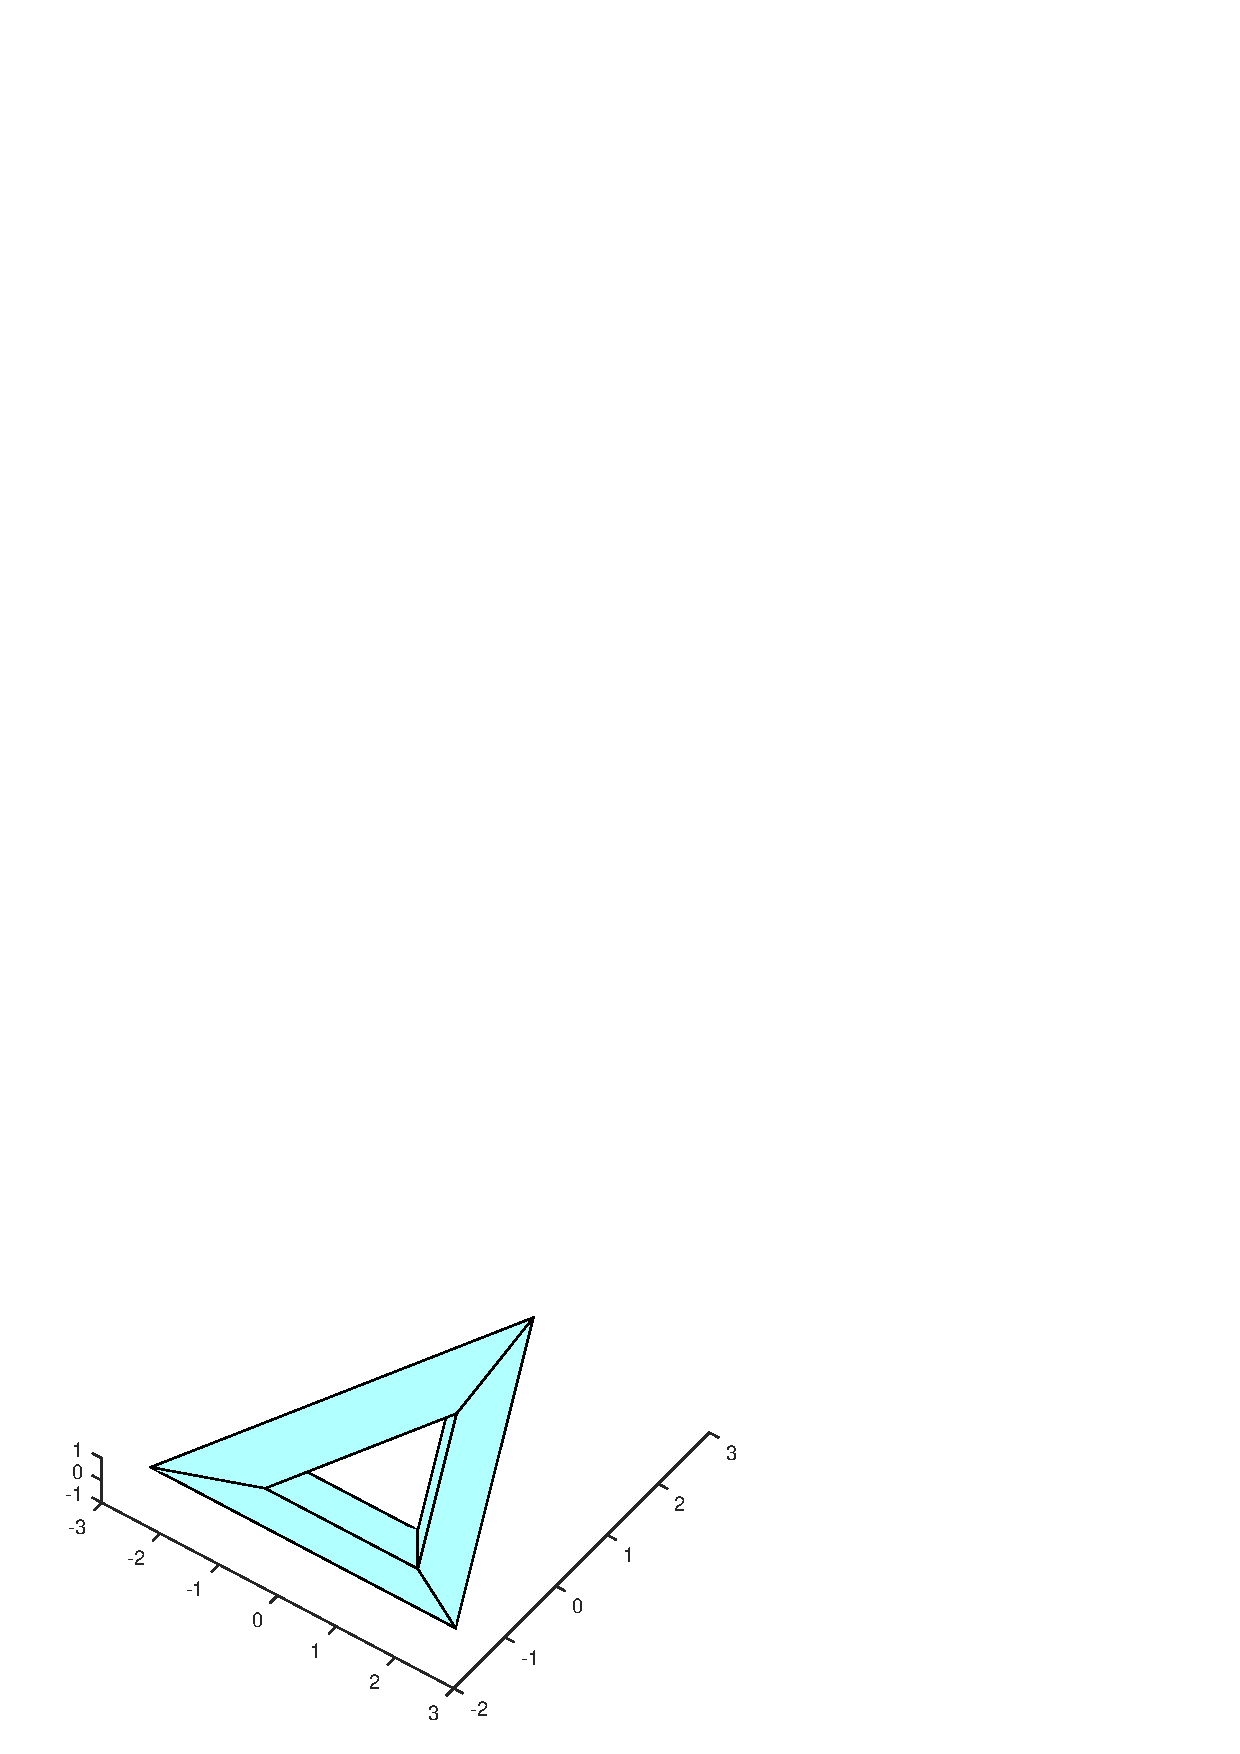
\includegraphics[width=5cm]{Pictures/NURBS/tikz/control_mesh.pdf}};
        
        \node at (3.5,3.5) [inner sep=0pt, scale = 0.5](N2)
        			{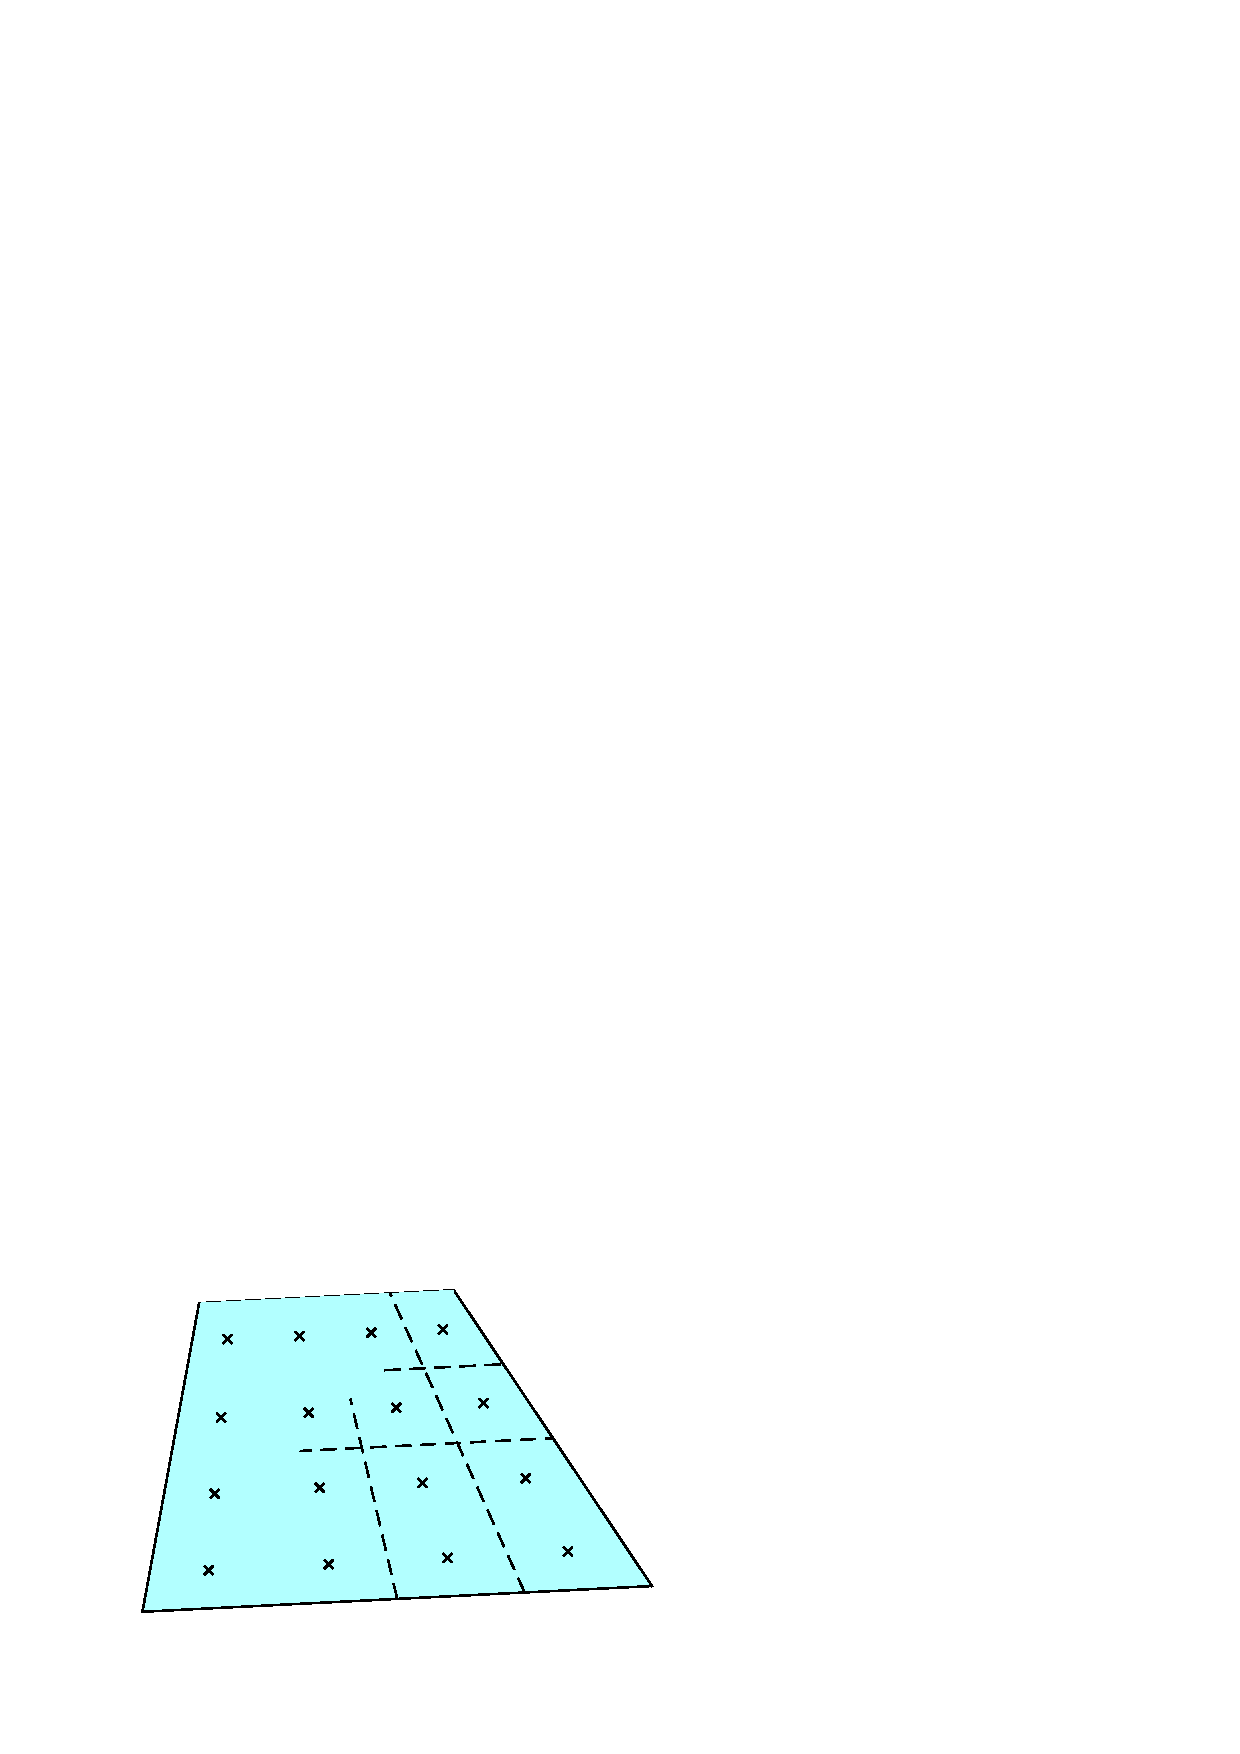
\includegraphics[width=5cm]{Pictures/NURBS/tikz/patch_points.pdf}};
        			                  
        \draw[thick,->] (N1) -- (N2);
        
        
        \node at (7,2)[inner sep=0pt, scale = 0.5](N3)
                  {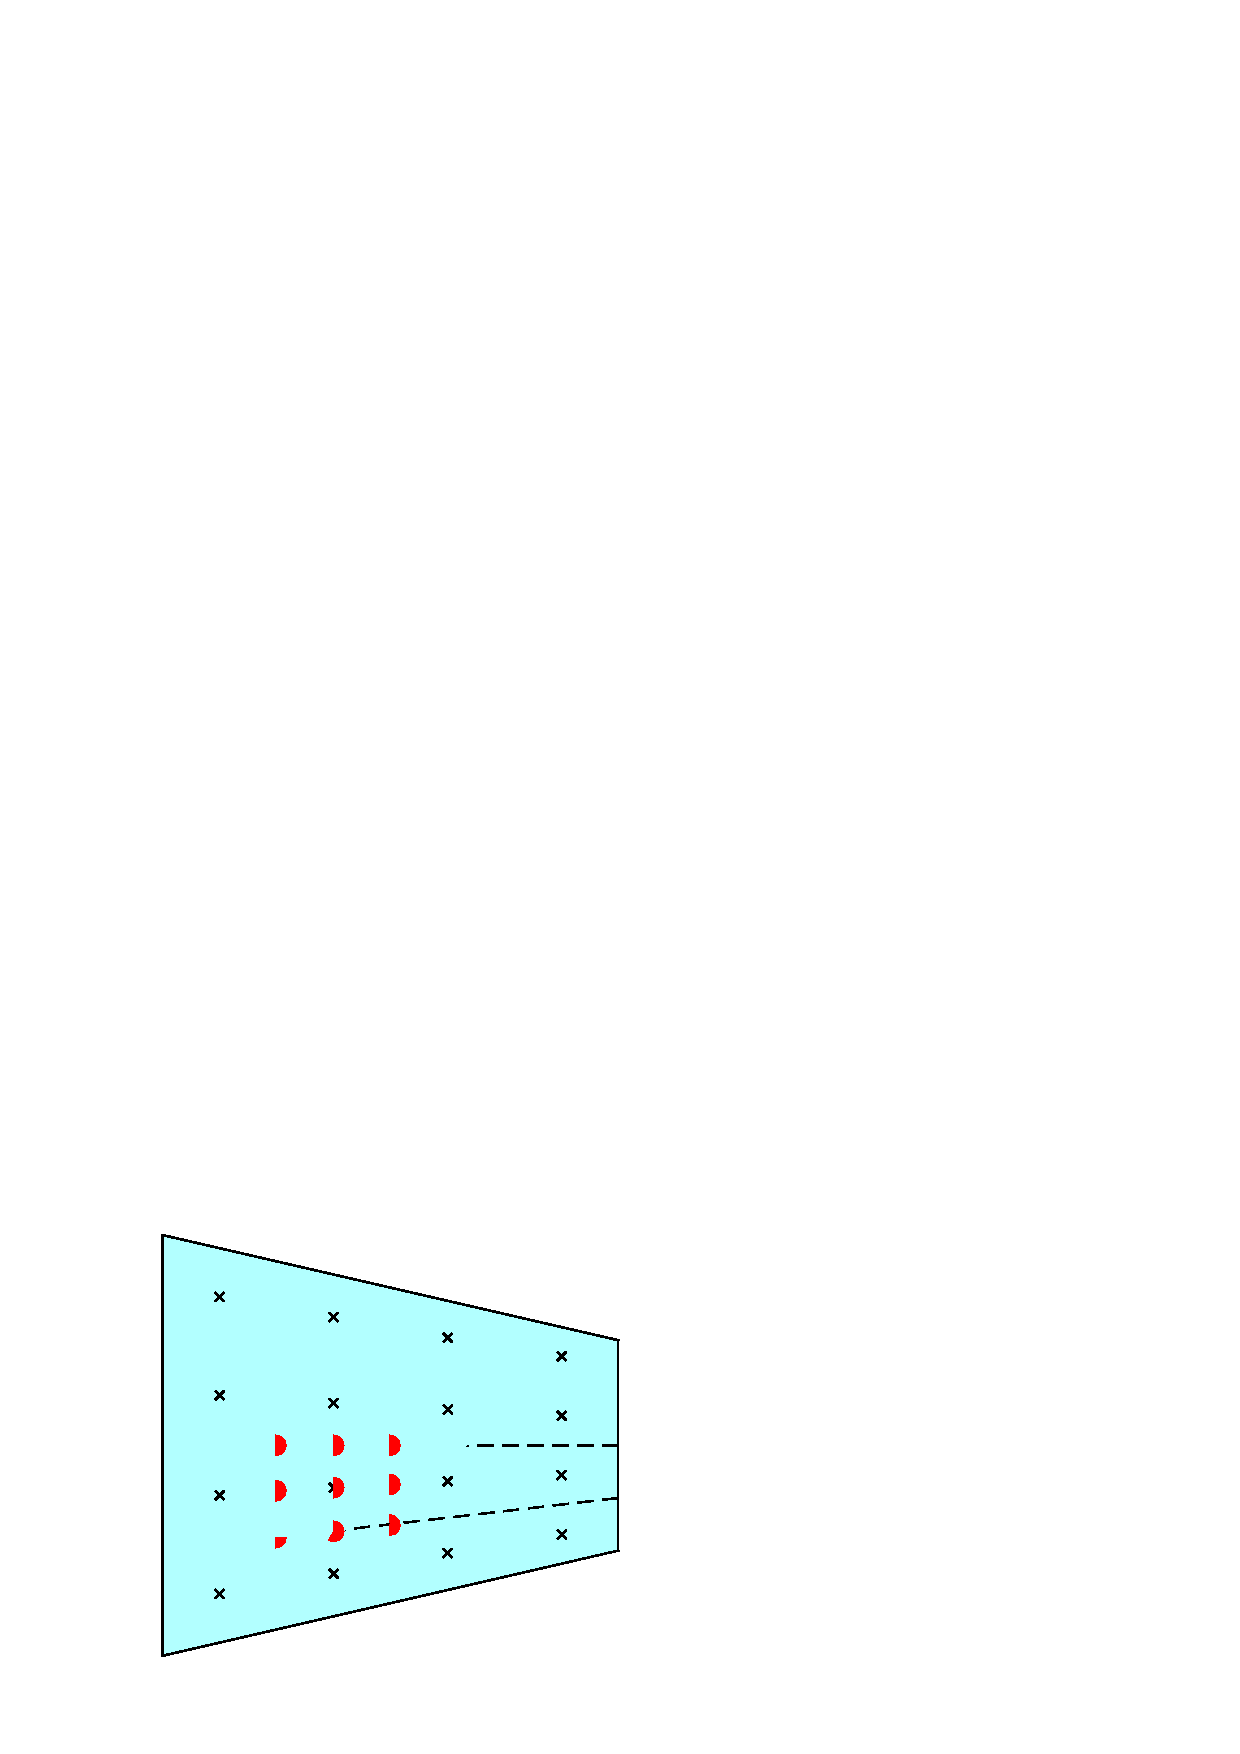
\includegraphics[width=5cm]{Pictures/NURBS/tikz/bezier_points.pdf}};
        \draw[thick,->] (N2) -- (N3);
        
        
        \node at (3.5, 0)[inner sep=0pt, scale = 0.5](N4)
                {\includegraphics[width=5cm]{Pictures/NURBS/tikz/bspline_patches.pdf}};
        \draw[thick,->] (N3) -- (N4);
        
        
        \node at (0, 0)[inner sep=0pt, scale = 0.5](N5)
                 {\includegraphics{Pictures/NURBS/tikz/torus_peters.pdf}};
        \draw[thick,->] (N4) -- (N5);
        
        \end{tikzpicture}
	\end{center}
\end{overlayarea}
%\textbf{{\color{red} According to Peters obtained surface is $G^{1}$ smooth}}
\end{frame}

\begin{frame}{Fitting Problem: Peters’ Scheme\textsuperscript{3}}
\vspace{-0.5cm}
\only<1>{
\begin{minipage}[t]{0.4\linewidth}
\begin{figure}
	\includegraphics[width=.88\textwidth]{Pictures/NURBS/mosquito_surface}
\end{figure}
\end{minipage}%
\hfill%
\begin{minipage}[t]{0.55\linewidth}
%\begin{block}{}
\vspace{0.27cm}
\begin{equation*}
||D - C(u, v) \ P||^2  \rightarrow min %\sum_{i=1}^{N}\norm{P_{i} - y_{i}V_{x}}^{2} \rightarrow min$$
\end{equation*}
%\end{block}
\end{minipage}}

\only<2>{
\begin{minipage}[t]{0.4\linewidth}
\begin{figure}
	\includegraphics[width=.88\textwidth]{Pictures/NURBS/mosquito_surface}
\end{figure}
\end{minipage}%
\hfill%
\begin{minipage}[t]{0.55\linewidth}
%\begin{block}{}
\begin{equation*}
||D - C(u, v) \ P||^2 + \textcolor{red}{\lambda ||0-C^{fair}P||}  \rightarrow min %\sum_{i=1}^{N}\norm{P_{i} - y_{i}V_{x}}^{2} \rightarrow min
\end{equation*}
%\end{block}
\end{minipage}}
\vspace{0.2cm}
\only<1>{
\begin{minipage}[t]{0.4\linewidth}
\begin{figure}
	\includegraphics[width=.88\textwidth]{Pictures/NURBS/ToCover}
\end{figure}
\end{minipage}%
\hfill%
\begin{minipage}[t]{0.55\linewidth}
\begin{block}{Notation}
$D$ - Data  points object to surface fitting\\
$C(u,v)$ - Control Point Matrix \\
$P$ - B-Spline Control Points \\
\end{block}
\end{minipage}}

\only<2>{
\begin{minipage}[t]{0.4\linewidth}
\begin{figure}
	\includegraphics[width=.88\textwidth]{Pictures/NURBS/MosquitoNo}
\end{figure}
\end{minipage}%
\hfill%
\begin{minipage}[t]{0.55\linewidth}
\begin{block}{Notation}
$D$ - Data  points object to surface fitting\\
$C(u,v)$ - Control Point Matrix \\
$P$ - B-Spline Control Points \\
\color{red}{$C^{fair}$ - Fairness coefficients}
\end{block}
\end{minipage}}

\end{frame}


\subsection{Back to CAD}
%  \begin{frame}
%  \frametitle{Contents}
%  \tableofcontents[currentsubsection]
%  \end{frame}
\begin{frame}{Recovery of Optimized Geometry}
	\begin{minipage}[t]{0.5\linewidth}
		\begin{block}{Geometry reconstruction}
			\begin{itemize}
				\item Surface patches constructed using data points from Peters' scheme \\
				\item Patches sewed together using FreeCAD to form a geometry \\
			\end{itemize}
		\end{block}
		\begin{block}{Post-processing}
			\begin{itemize}
				\item Non-changing regions restored \\
				\item Solution restricted to desired limits \\
				\item Final export done as a STEP file
			\end{itemize}
		\end{block}
	\end{minipage}
	\hfill
	\begin{minipage}[t]{0.45\linewidth}
		\vspace{-0.25cm}
		\begin{figure}
			\includegraphics[width=.88\textwidth]{Pictures/SecondHalf/Back2CAD1}
		\end{figure}
		\vspace{-0.75cm}
		\begin{center}
			$\downarrow$
		\end{center}
		\vspace{-0.6cm}
		\begin{figure}
			\includegraphics[width=.88\textwidth]{Pictures/SecondHalf/Back2CAD2}
		\end{figure}
		\vspace{-0.75cm}
		\begin{center}
			$\downarrow$
		\end{center}
		\vspace{-0.6cm}
		\begin{figure}
			\includegraphics[width=.88\textwidth]{Pictures/SecondHalf/Back2CAD3}
		\end{figure}
	\end{minipage}
\end{frame}


\section{Summary \& Outlook}
%  \begin{frame}
%  \setcounter{tocdepth}{1}
%  \frametitle{Contents}
%  \tableofcontents[hideallsubsections,currentsection]
%  \end{frame}
\begin{frame}{Third Milestone's achievements}
%\begin{variableblock}{What's done?}{bg=cyan,fg=white}{bg=white,fg=black}
%{



\begin{itemize}
	\item[\textcolor{green}{\Checkmark}] Fully integrated pipeline 
	
	\item[\textcolor{green}
	{\Checkmark}] Boolean operation support
		
	\item[\textcolor{green}
	{\Checkmark}] GUI for user interaction
	
	\item[\textcolor{green}
	{\Checkmark}] Fairness functional to control Peters' scheme smoothness
	
		\item[\textcolor{green}
	{\Checkmark}] Conversion back to CAD
	
	\item[\textcolor{green}
	{\Checkmark}] Test Cases


\end{itemize}

\end{frame}

\begin{frame}{Outlook \& future work}
\begin{itemize}
\item Make surface reconstruction more robust
\item Improve parameter estimation
\begin{itemize}
\item[--] complexity of algorithm 
\item[--] accuracy of result
\end{itemize}
\item Determine approximation error for our algorithm
\begin{itemize}
\item[--] Topology checks
\item[--] Accuracy estimates
\end{itemize}
\item Develop a fully adaptive scheme
\item Exchange ToPy with a faster solution
\end{itemize}
\end{frame}

\begin{frame}{But what can we currently achieve?}
\begin{figure}
%\vspace{-.7cm}	
%\hspace{-2cm}
		\includegraphics[width=1\linewidth]{Pictures/SecondHalf/TestCases.png}
		\end{figure}

\end{frame}
\begin{frame}
\begin{figure}

\vspace{-.7cm}	
\hspace{-2cm}		\includegraphics[width=1.2\linewidth]{Pictures/animations/animation_10.png}
		\end{figure}

\end{frame}





%%%%%%%%%%%%%%%%%%%%%%%%%%%%%%%%%%%%%%%
%%%OLD SLIDES

%\begin{frame}{What is next?}
%\begin{variableblock}{What's done?}{bg=cyan,fg=white}{bg=white,fg=black}
%{
%\begin{itemize}

%\item<+-> Topology Optimization
%\begin{itemize}
%	\item[\textcolor{green}{\Checkmark}] Pipeline from CAD model to optimized voxel model
%	\item[\textcolor{green}{\Checkmark}] User input of boundary conditions
%	\item[\textcolor{black}{\VarClock}] Support for complex geometries
%	\item[\textcolor{red}{\XSolidBrush}] GUI for user interaction
%\end{itemize}

%\item<+-> Surface Extraction
%\begin{itemize}
%	\item[\textcolor{green}{\Checkmark}] Dual Contouring for simple geometries
%	\item[\textcolor{green}{\Checkmark}] Provide necessary data for Surface Fitting
%	\item[\textcolor{black}{\VarClock}] Interfaces
	%\item[\textcolor{red}{\XSolidBrush}] Adaptive and topology safe Dual Contouring
%\end{itemize}

%\item<+-> Surface Fitting
%\begin{itemize}
	%\item[\textcolor{green}{\Checkmark}] B--spline fitting using least squares
	%\item[\textcolor{green}{\Checkmark}] Smooth connection of patches using Peters' scheme
	%\item[\textcolor{red}{\XSolidBrush}] Conversion back to CAD
%\end{itemize}
%\end{itemize}
%}
%\end{variableblock}
%\end{frame}

















%\section*{Thank You}
%\begin{frame}{Thank you for your attention!}
	\begin{figure}
		\scalebox{0.14}{\includegraphics{Pictures/1CAD.pdf}}
		\scalebox{0.14}{\includegraphics{Pictures/2STL.pdf}}
		\scalebox{0.14}{\includegraphics{Pictures/3VOX.pdf}}
		\scalebox{0.14}{\includegraphics{Pictures/4TPD.pdf}}
		\scalebox{0.14}{\includegraphics{Pictures/5TOPOPT.pdf}}
		\scalebox{0.14}{\includegraphics{Pictures/6TOPYOUT.pdf}}
		\scalebox{0.14}{\includegraphics{Pictures/7MC.pdf}}
	\end{figure}
	\begin{figure}
	\includegraphics[scale=0.2]{Pictures/TheArc.png}
	\end{figure}
\end{frame}

\section*{Literature}
\begin{frame}{Literature}
\begin{itemize}
\item \textbf{William Hunter.} "Predominantly solid-void three-dimensional topology optimisation using open source software"
\item \textbf{Gerrit Becker, Michael Sch\"afer, Antony Jameson.} "An advanced NURBS fitting procedure for post-processing of grid-based shape optimizations"
\item \textbf{Matthias Eck, Hugues Hoppe.} "Automatic Reconstruction of B-Spline Surfaces of Arbitrary Topological Type"
\item \textbf{Tao Ju, Frank Losasso, Scott Schaefer, Joe Warren.} "Dual contouring of hermite data"
\end{itemize}
\end{frame}

\section*{Theory}
\begin{frame}{Projection and Parametrization on arbitrary quads}
\begin{overlayarea}{\textwidth}{.15 \textheight}
\begin{enumerate}
\item<1-> find least squares plane approximating quad
\item<2-> projection of datapoint onto plane
\item<3-> find corresponding parameters $\left[u,v\right] \in \left[0,1\right]^2$
\end{enumerate}
\end{overlayarea}
\begin{overlayarea}{\textwidth}{.85 \textheight}
\only<1>{
\begin{columns}
\column{.3\textwidth}
\begin{figure}
\includegraphics[width = \textwidth]{Pictures/BackupSlidesProjection/nonPlaneQuads.png}
\caption{DC sphere}
\end{figure}
\column{.3\textwidth}
\begin{figure}
\includegraphics[width = \textwidth]{Pictures/BackupSlidesProjection/withPlaneQuads.png}
\caption{with plane quads}
\end{figure}
\end{columns}
}
\begin{columns}
\column{.35\textwidth}

\begin{overlayarea}{\textwidth}{\textheight}
\begin{figure}
\only<2-3>{
\tdplotsetmaincoords{60}{110}
\begin{tikzpicture}[scale = 1.5,tdplot_main_coords]
\coordinate (O) at (-1,-1,0);
\coordinate[dot] (A) at (0,0,0);
\coordinate[dot] (B) at (1,0,0);
\coordinate[dot] (C) at (1.2,1.5,0);
\coordinate[dot] (D) at (0,1,0);
\coordinate (P1) at (.5,.4,1);
\coordinate (P2) at (1,1,1);
\coordinate (Q1) at (.5,.4,0);
\coordinate (Q2) at (1,1,0);

\draw[thick,->] (O) -- ($(O)+(.5,0,0)$) node[anchor=north east]{$x$};
\draw[thick,->] (O) -- ($(O)+(0,.5,0)$) node[anchor=north west]{$y$};
\draw[thick,->] (O) -- ($(O)+(0,0,.5)$) node[anchor=south]{$z$};

\draw[thick] (A) -- (B) -- (C) -- (D) -- (A);

\only<2-3>{
\draw (P1) node[thick,cross,red,label = {$P_1$}] {};
\draw[red,dashed] (P1) -- (Q1);
\draw (Q1) node[thick,cross,red] {};
}
\only<3>{
\draw (P2) node[thick,cross,red,label = {$P_2$}] {};
\draw[red,dashed] (P2) -- (Q2);
\draw (Q2) node[thick,cross,red] {};
\draw[black,dashed] (B) -- (D);
}
\draw (A) node[label = left:{$A$}]{};
\draw (B) node[label = left:{$B$}]{};
\draw (C) node[label = right:{$C$}]{};
\draw (D) node[label = right:{$D$}]{};
\end{tikzpicture}
}
\end{figure}
\end{overlayarea}

\column{.5\textwidth}
\begin{overlayarea}{\textwidth}{\textheight}
\only<2>{
\begin{block}{Coordinate transformation}
system with basis
\begin{equation*}
B_{BAD} = \left(
\begin{array}{ccc}
\vec{n} & \vec{AB} & \vec{AD}
\end{array}
\right)
\end{equation*}
yields
\begin{equation*}
\left(B_{BAD}\right)^{-1} P_1
=
\left(
\begin{array}{ccc}
d&u&v
\end{array}
\right)^T
\end{equation*}
\end{block}
}
\only<3>{
\begin{block}{Problem:}
\begin{itemize}
\item[\textcolor{green}{\Checkmark}] for $P_1$: $\left(u,v\right) = \left(0.5,0.4\right)$
\item[\textcolor{red}{\XSolidBrush}] for $P_2$: $\left(u,v\right) = \left(1,1\right)$
\end{itemize}
\end{block}

\begin{block}{Solution:}
\begin{enumerate}
\item if we get $u+v > 1$
\item use $B_{BCD}$ instead of $B_{BAD}$
\item set $u=1-u$, $v=1-v$
\end{enumerate}
\end{block}

}
\end{overlayarea}
\end{columns}
\end{overlayarea}
\end{frame}

\end{document}
